%Erstemal, dass ich mit Latex arbeite, daher bitte nicht schlagen :D
\documentclass[a4paper, 11pt]{report}

\usepackage[ngerman]{babel}
\usepackage[latin1]{inputenc}
\usepackage{graphicx}
\usepackage{amsmath}
\usepackage{txfonts}
\usepackage{pstricks}

\newcommand{\N}{\varmathbb{N}}
\newcommand{\Z}{\varmathbb{Z}}
\newcommand{\Q}{\varmathbb{Q}}
\newcommand{\R}{\varmathbb{R}}
\newcommand{\C}{\varmathbb{C}}
\begin{document}

\tableofcontents

\newpage

\chapter{Einf�hrung}
\section{Inhalt}
�bertragung (Speicherung) von Daten:\\
Schutz vor:
\begin{itemize}
	\item[-] zuf�lligen oder systematischen (physikalischen bedingten) St�rungen
	\item[-] Abh�ren, absichtliche Ver�nderung von Dritten (Kryptologie / Verschl�sselung)
\end{itemize}
\underline{Kryptologie:}
\begin{itemize}
	\item[-] symmetrische Verfahren
	\item[-] asymmetrische Verfahren (Public-Key Verfahren)
	\item[-] Authentifizierung
	\item[-] Signaturen
\end{itemize}
\underline{Codierungstheorie}
\begin{itemize}
	\item[-] Fehlererkennung und Fehlerkorrektur
	\item[-] lineare Blockcodes
	\item[-] Decodierverfahren
\end{itemize}

\newpage

\chapter{Kryptologie}

\section{Grundbegriffe und einfache Verfahren}
\begin{figure}[h]
	\centering
	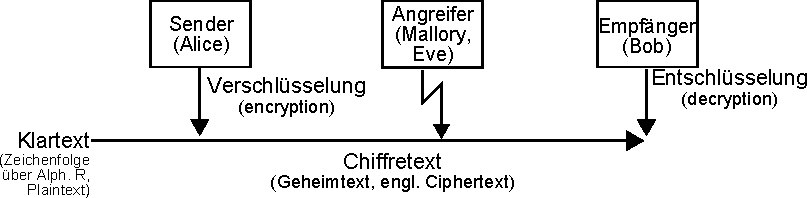
\includegraphics{./img/krypto_schaubild.pdf}
	\caption{Schaubild der Kryptologie}
	\label{img:Schaubild}
\end{figure}

\subsection{Verschl�sselung erfordert}
\begin{itemize}
	\item[-] Verschl�sselungsverfahren, Algorithmus (Funktion)
	\item[-] Schl�ssel $k_{e}$ (encryption key)
\end{itemize}
$E(m,k_e)=c$\\
$E$=Verschl.Fkt., $m$=Klartext, $c$=Chiffretext\\
$E(m_1,k_e)\neq E(m,k_e)$ f�r $m_1\neq m_2$\\
$D(c,k_d)=m$\\
($k_d$ zu $k_e$ geh�riger Dechiffrierschl�ssel!)\\

$k_d=k_e$ (oder $k_d$ leicht aus $k_e$ zu berechnen):\\
\underline{symmetrisches Verschl.verf.}, ansonsten \underline{asymm. Verschl.verf.}. Ist $k_d$ nur sehr schwer (oder garnicht) zu $k_e$ berechenbar, so kann $k_e$ ver�ffentl. werden:\\
\underline{Public-Key-Verfahren}.
\subsection{Beispiel f�r (nicht sicheres) symm. Verfahren}
\begin{itemize}
	\item[a)] $R=S=\left\{0,1,\ldots,25\right\}$\\
	Verfahren: Verschiebechiffre\\
	Schl�ssel: $i \in \left\{0,1,\ldots,25\right\}$\\
	Verfahren $ x \in \R \longrightarrow x+i$ mod $26=y$\\
	$y\longmapsto y-i$ mod $26 = y$\\
	$m=x_1 ... x_2 \longrightarrow  c = (x_1 + i$ mod $26) \ldots (x_n +i$ mod $ 26)$, $E(m,i)$\\
	Unsicher, weil Schl�sselmenge klein ist (Brute Force Angriff).
	\item[b)] R,S, Schl�sselmenge=Menge aller Permutationen von $\left\{1,\ldots,25\right\}=S_{26}$\\
	Verschl.: W�hle Permuation $\pi$\\
	$x \in \R \longrightarrow \pi (x)=y$\\
	Entschl.: $y \longrightarrow \pi^{-1}(y)=x$\\
	$m=x_1 \ldots x_r \rightarrow c=\pi(x_1)\ldots\pi(x_r)$\\
	$\begin{pmatrix}
  0 & 1 & 2 & \ldots & 25 \\
  3 & 17 & 4 & \ldots & 13
	\end{pmatrix}
	\longrightarrow \pi(0)=3$, u.s.w.\\
	Anzahl der Permutationen: $\left|{S_{26}}\right|=26!\approx4\cdot10^{26} \longrightarrow$ Brute-Force Angriff nicht mehr m�glich! \\
	Warum? Man muss im Schnitt 50\% der Permutationen testen. Angenommen man k�nnte $10^12$ Perm. pro Sekunde testen.\\
	Aufwand: $2\cdot10^{14}$ Sekunden $\approx 6.000.000$ Jahre\\
	Trotzdem unsicher!\\
	Grund: Charakteristiches H�ufigkeitsverteilung von Buchstaben in nat�rlichspr. Texten.
\end{itemize}
Verfahren beinhalten viele Verschl�sselungsm�glichkeiten, abh�ngig von der Auswahl des Schl�ssels.\\
Verfahren bekannt, aber Schl�ssel $k_d$ geheim!\\
\subsection{Prinzip von Kerkhoffs (1835-1903)}
Sicherheit eines Verschl�sselungsverfahren darf nicht von der Geheimhaltung des Verfahrens, sondern nur von der Geheimhaltung des verwendeten Schl�ssels abh�ngen!
%
%	Ende Stunde vom 29.10.2009
%
\newpage
\end{document}
